	\section{Цель работы:}
		Разработать систему нечеткого логического вывода (например, систему поддержки принятия решений, основанную на нечеткой логике).
	\section{Порядок выполенения работы:}
	
		\subsection{Предметная область:}
		Врачебная диагностика пациента.
		
		\subsection{Задача:}
		Определить степень тяжести состояния среднего пациента в зависимости от показателей давления, частоты сердечных сокращений и частоты дыхательных движений.
		\subsection{Описание входных данных с помощью векторов лингвистических переменных:}
			\subsubsection{Систолическая составляющая давления}
				\textit{Название переменной}: $ \omega = "\text{систалическое давление}" $
				
				\textit{Терм-множество значений:}
				\begin{itemize}
					\item $ T_1 = "\text{нормальное}" $
					\item $ T_2 = "\text{менее нормальное}" $
					\item $ T_3 = "\text{наименее нормалное}" $
				\end{itemize}
			
				\textit{Носитель:} $ U = [ 0, 200 ] $
					
				\textit{Синтаксическое правило:} Уровень систаличекого давления пациента.
					
				\textit{Семантическое правило:} определяется функциями принадлежности, для значения $T_1 - \mu_1(U)$, для $T_2 - \mu_2(U)$, для $T_3 - \mu_3(U)$. Причем первая из них отвечает нечеткому подмножеству $M_1$, вторая – $M_2$, третья – $M_3$
			\subsubsection{Диастолическая составляющая давления}
				\textit{Название переменной}: $ \omega = "\text{диастолическое давление}" $
				
				\textit{Терм-множество значений:}
				\begin{itemize}
					\item $ T_1 = "\text{нормальное}" $
					\item $ T_2 = "\text{менее нормальное}" $
					\item $ T_3 = "\text{наименее нормалное}" $
				\end{itemize}
				
				\textit{Носитель:} $ U = [ 0, 200 ] $
				
				\textit{Синтаксическое правило:} Уровень диастолического давления пациента.
				
				\textit{Семантическое правило:} определяется функциями принадлежности, для значения $T_1 - \mu_1(U)$, для $T_2 - \mu_2(U)$, для $T_3 - \mu_3(U)$. Причем первая из них отвечает нечеткому подмножеству $M_1$, вторая – $M_2$, третья – $M_3$
		
			\subsubsection{Частота сердечных сокращений}
				\textit{Название переменной}: $ \omega = "\text{пульс}" $
				
				\textit{Терм-множество значений:}
				\begin{itemize}
					\item $ T_1 = "\text{нормальный}" $
					\item $ T_2 = "\text{нитевидный}" $
				\end{itemize}
				
				\textit{Носитель:} $ U = [ 0, 200 ] $
				
				\textit{Синтаксическое правило:} Уровень диастолического давления пациента.
				
				\textit{Семантическое правило:} определяется функциями принадлежности, для значения $T_1 - \mu_1(U)$, для $T_2 - \mu_2(U)$. Причем первая из них отвечает нечеткому подмножеству $M_1$, вторая – $M_2$.
				
			\subsubsection{Частоты дыхательных движений}
				\textit{Название переменной}: $ \omega = "\text{частота дыхания}" $
				
				\textit{Терм-множество значений:}
				\begin{itemize}
					\item $ T_1 = "\text{нормальная}" $
					\item $ T_2 = "\text{высокая}" $
					\item $ T_3 = "\text{очень высокая}" $
					\item $ T_4 = "\text{экстремальная}" $
				\end{itemize}
				
				\textit{Носитель:} $ U = [ 10, 70 ] $
				
				\textit{Синтаксическое правило:} Уровень диастолического давления пациента.
				
				\textit{Семантическое правило:} определяется функциями принадлежности, для значения $T_1 - \mu_1(U)$, для $T_2 - \mu_2(U)$, для $T_3 - \mu_3(U)$, для $T_4 - \mu_4(U)$. Причем первая из них отвечает нечеткому подмножеству $M_1$, вторая – $M_2$, третья – $M_3$, четвёртая – $M_4$
				
		\subsection{Описание выходных данных с помощью векторов лингвистических переменных:}
		
			\subsubsection{Тяжесть состояния пациента}
				\textit{Название переменной}: $ \omega = "\text{состояние}" $
				
				\textit{Терм-множество значений:}
				\begin{itemize}
					\item $ T_1 = "\text{удовлетворительное}" $
					\item $ T_2 = "\text{средней тяжести}" $
					\item $ T_3 = "\text{тяжёлое}" $
					\item $ T_4 = "\text{крайне тяжёлое}" $
				\end{itemize}
				\textit{Носитель:} $ U = [ 0\%, 100\% ] $
				
				\textit{Синтаксическое правило:} Уровень диастолического давления пациента.
				
				\textit{Семантическое правило:} определяется функциями принадлежности, для значения $T_1 - \mu_1(U)$, для $T_2 - \mu_2(U)$, для $T_3 - \mu_3(U)$, для $T_4 - \mu_4(U)$. Причем первая из них отвечает нечеткому подмножеству $M_1$, вторая – $M_2$, третья – $M_3$, четвёртая – $M_4$
				
		\subsection{Построение графиков для всех описанных лингвистических переменных:}
			\begin{figure}[h!]
				\center{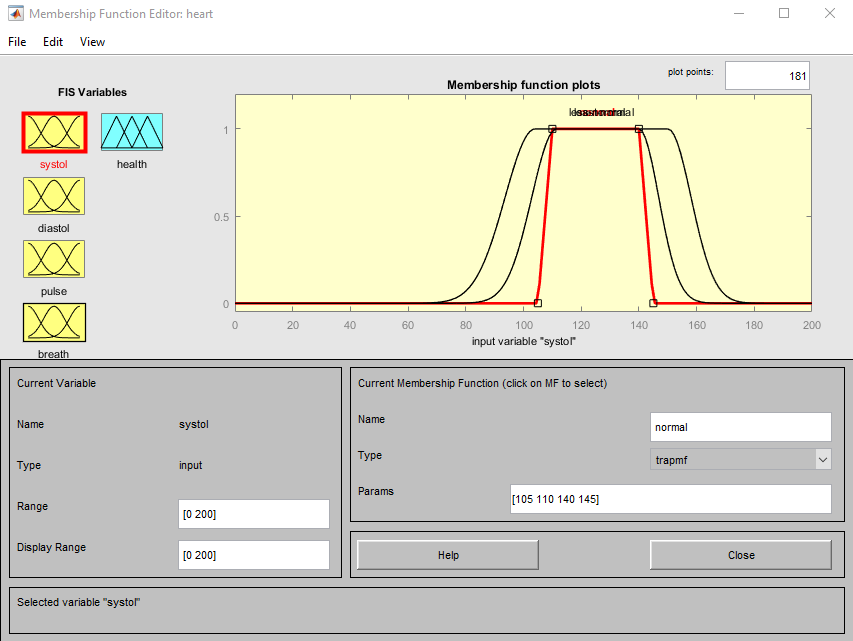
\includegraphics[width=0.7\paperwidth]{v1}}
				\caption{Систолическая составляющая давления}
				\label{systol}
			\end{figure}
		
			\begin{figure}[h!]
				\center{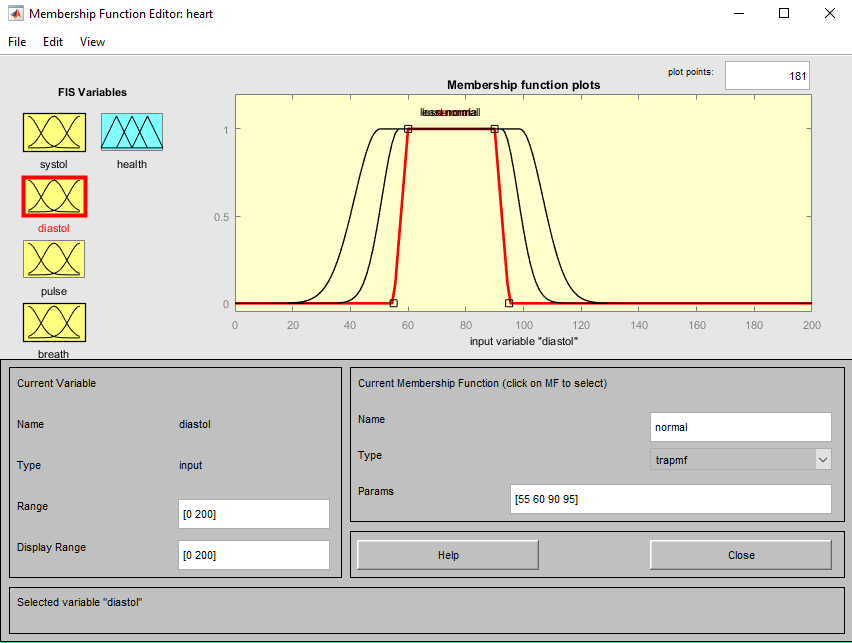
\includegraphics[width=0.7\paperwidth]{v2}}
				\caption{Диастолическая составляющая давления}
				\label{diastol}
			\end{figure}
		
			\begin{figure}[h!]
				\center{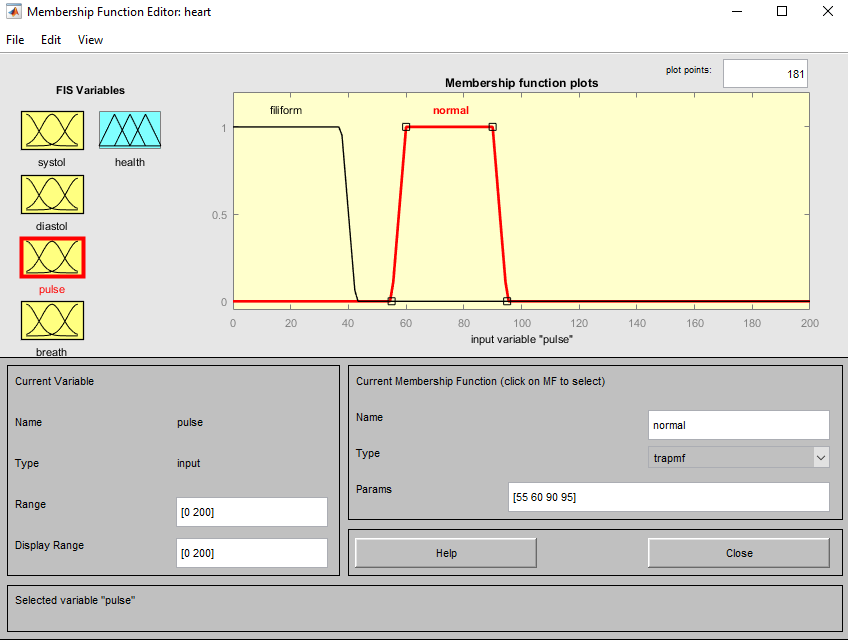
\includegraphics[width=0.7\paperwidth]{v3}}
				\caption{Частота сердечных сокращений}
				\label{pulse}
			\end{figure}
		
			\begin{figure}[h!]
				\center{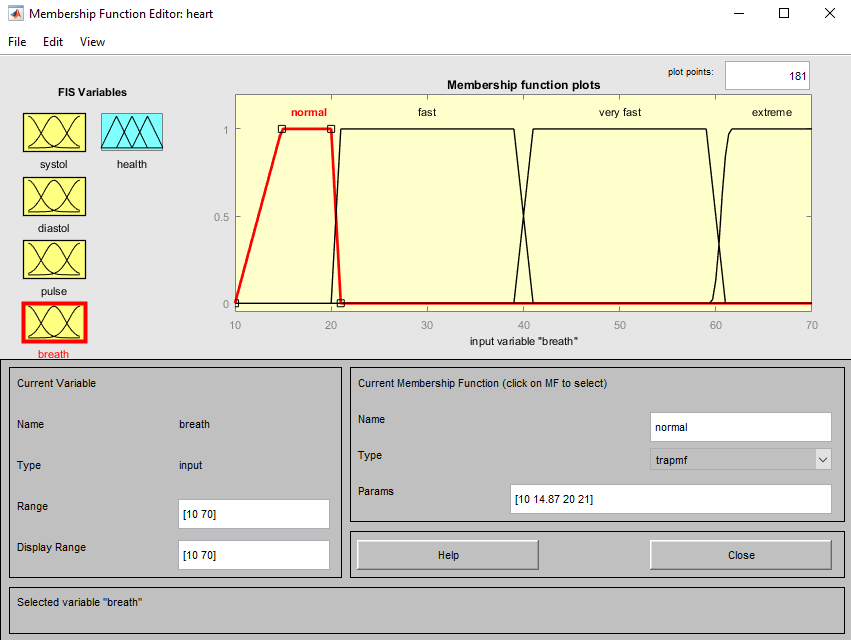
\includegraphics[width=0.7\paperwidth]{v4}}
				\caption{Частота дыхательных движений}
				\label{breath}
			\end{figure}
		
			\begin{figure}[h!]
				\center{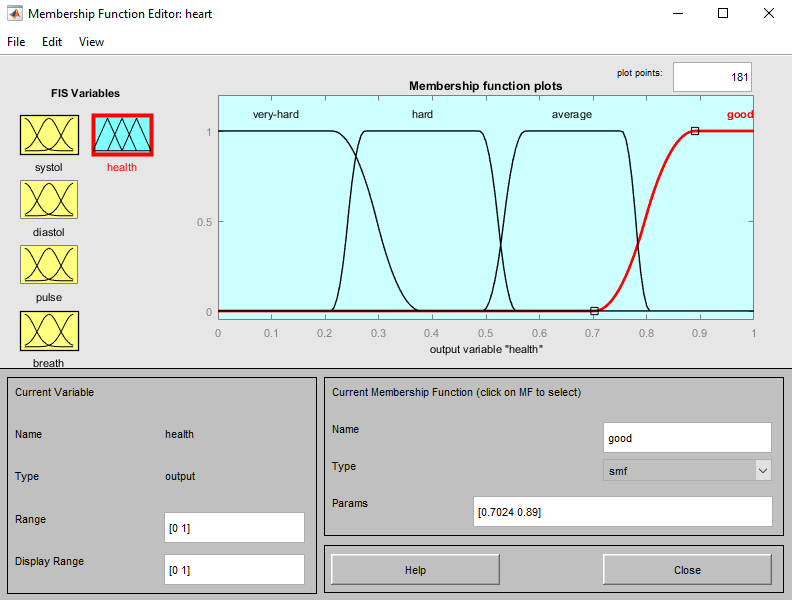
\includegraphics[width=0.7\paperwidth]{r1}}
				\caption{Тяжесть состояния пациента}
				\label{health}
			\end{figure}
		
		\subsection{Формирование базы правила «Если-то»}
			\begin{enumerate}
				\item \underline{\textbf{Если}} ($"\text{диастолическое давление}"$ = $"\text{нормальное}"$) и ($"\text{систалическое давление}"$ =  $"\text{нормальное}"$) и ( $"\text{пульс}"$ =  $"\text{нормальный}"$) и ( $"\text{частота дыхания}"$ =  $"\text{нормальная}"$), \underline{\textbf{то}} ($"\text{состояние}"$ =  $"\text{удовлетворительное}"$)
				
				\item \underline{\textbf{Если}} ( $"\text{частота дыхания}"$ =  $"\text{экстремальная}"$), \underline{\textbf{то}} ($"\text{состояние}"$ =  $"\text{крайне тяжёлое}"$)
				
				\item \underline{\textbf{Если}} ( $"\text{частота дыхания}"$ =  $"\text{\textbf{не} экстремальная}"$), \underline{\textbf{то}} ($"\text{состояние}"$ =  $"\text{\textbf{не} крайне тяжёлое}"$)
				
				\item \underline{\textbf{Если}} ( $"\text{частота дыхания}"$ =  $"\text{очень высокая}"$), \underline{\textbf{то}} ($"\text{состояние}"$ =  $"\text{тяжёлое}"$)

				\item \underline{\textbf{Если}} ( $"\text{пульс}"$ =  $"\text{нитевидный}"$) или $"\text{частота дыхания}"$ =  $"\text{\textbf{не} экстремальная}"$, \underline{\textbf{то}} ($"\text{состояние}"$ =  $"\text{\textbf{не} удовлетворительное}"$)
				
				\item \underline{\textbf{Если}} ( $"\text{пульс}"$ =  $"\text{нитевидный}"$), \underline{\textbf{то}} ($"\text{состояние}"$ =  $"\text{\textbf{не} средней тяжести}"$)
								
				\item \underline{\textbf{Если}} ( $"\text{пульс}"$ =  $"\text{нитевидный}"$) и ( $"\text{частота дыхания}"$ =  $"\text{\textbf{не} экстремальная}"$), \underline{\textbf{то}} ($"\text{состояние}"$ =  $"\text{тяжёлое}"$)
				
				\item \underline{\textbf{Если}} ($"\text{диастолическое давление}"$ = $"\text{\textbf{не} менее нормальное}"$) и ( $"\text{частота дыхания}"$ =  $"\text{\textbf{не} экстремальная}"$), \underline{\textbf{то}} ($"\text{состояние}"$ =  $"\text{тяжёлое}"$)
				
				\item \underline{\textbf{Если}} ($"\text{систолическое давление}"$ = $"\text{\textbf{не} менее нормальное}"$) и ( $"\text{частота дыхания}"$ =  $"\text{\textbf{не} экстремальная}"$), \underline{\textbf{то}} ($"\text{состояние}"$ =  $"\text{тяжёлое}"$)
				
				\item \underline{\textbf{Если}} ($"\text{диастолическое давление}"$ = $"\text{\textbf{не} менее нормальное}"$) или ($"\text{систалическое давление}"$ =  $"\text{\textbf{не} менее нормальное}"$) или ( $"\text{пульс}"$ =  $"\text{\textbf{не} нормальный}"$) или ( $"\text{частота дыхания}"$ =  $"\text{высокая}"$), \underline{\textbf{то}} ($"\text{состояние}"$ =  $"\text{средней тяжести}"$)

			\end{enumerate}
		
		\subsection{Нечеткий логический вывод по алгоритму Мамдани}
		
			Логическая операция И имеет следующие реализации:
			\begin{itemize}
				\item \textbf{min} – минимум;
				\item \textbf{prod} – умножение;
			\end{itemize}
	
			Логическая операция ИЛИ имеет следующие реализации:
			\begin{itemize}
				\item \textbf{max} – умножение;
				\item \textbf{probor} - вероятностное ИЛИ.
			\end{itemize}
		
			Импликация имеет следующие реализации:
			\begin{itemize}
				\item \textbf{min} – минимум;
				\item \textbf{prod} – умножение;
			\end{itemize}
	
			Операции объединения функций принадлежности выходной переменной имеют следующие реализации:
			\begin{itemize}
				\item	\textbf{max} – максимум;
				\item	\textbf{sum} – сумма;
				\item	\textbf{probor} - вероятностное ИЛИ.
			\end{itemize}
		
			Можно использовать следующие методы дефаззификации:
			\begin{itemize}
				\item	\textbf{centroid} – центр тяжести;
				\item	\textbf{bisector} –медиана;
				\item	\textbf{lom} – наибольший из максимумов;
				\item	\textbf{som} – наименьший из максимумов;
				\item	\textbf{mom} – среднее из максимумов.
			\end{itemize}
			
			Сравним методы дефаззификации при указанных на рис. \ref{params} параметрах.
			\begin{figure}[h!]
				\center{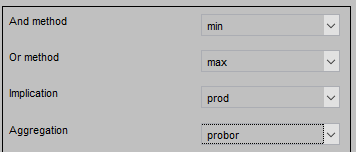
\includegraphics[width=0.7\paperwidth]{params}}
				\caption{Выбранные реализации операций.}
				\label{params}
			\end{figure}
			
			
			\begin{figure}[h!]
				\center{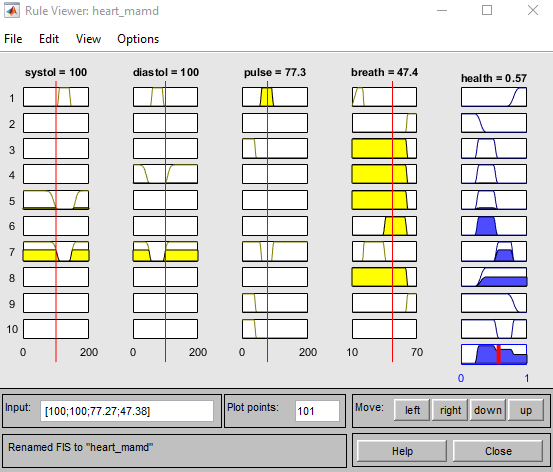
\includegraphics[width=0.6\paperwidth]{mamd_centr}}
				\caption{Метод центра тяжести.}
			\end{figure}
		
			\begin{figure}[h!]
				\center{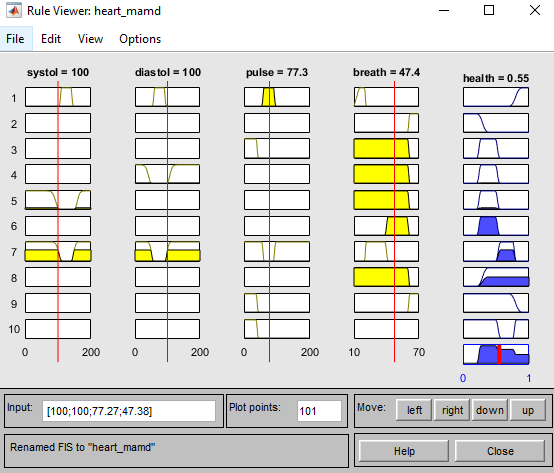
\includegraphics[width=0.6\paperwidth]{mamd_bisector}}
				\caption{Метод биссектрисы площади.}
			\end{figure}
			
			\begin{figure}[h!]
				\center{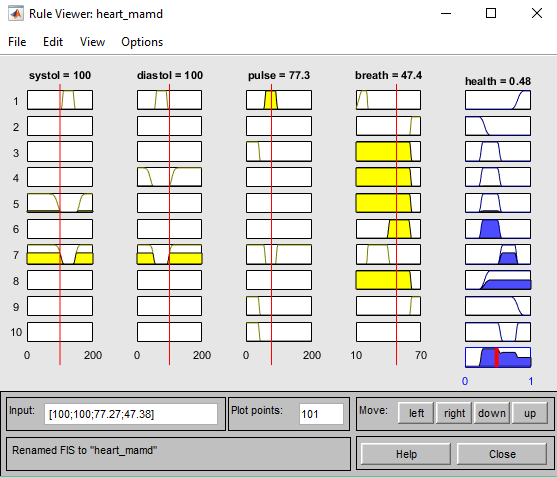
\includegraphics[width=0.6\paperwidth]{mamd_lom}}
				\caption{Метод наибольшего из максимумов.}
			\end{figure}
		
			\begin{figure}[h!]
				\center{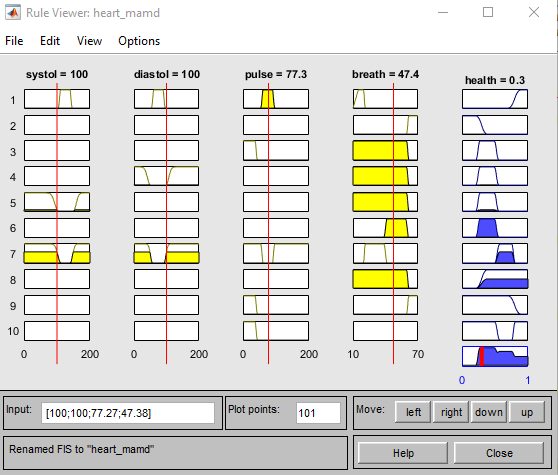
\includegraphics[width=0.6\paperwidth]{mamd_som}}
				\caption{Метод наименьшего из максимумов.}
			\end{figure}
			
			\begin{figure}[h!]
				\center{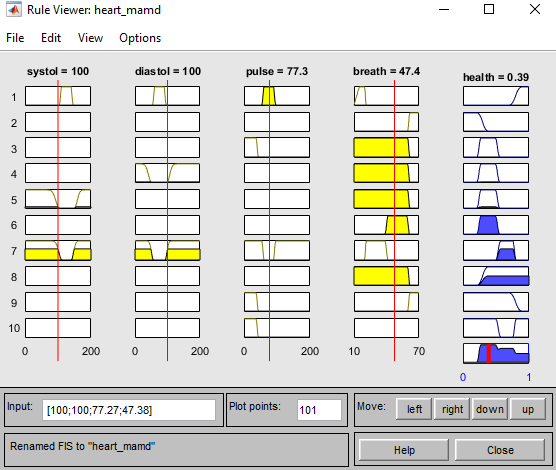
\includegraphics[width=0.6\paperwidth]{mamd_mom}}
				\caption{Метод среднего из максимумов.}
			\end{figure}
		
		\FloatBarrier
		\clearpage
		
		\subsection{Нечеткий логический вывод по алгоритму Сугено}
		
		Можно использовать следующие методы дефаззификации:
			\begin{itemize}
				\item \textbf{wtaver} – взвешенное среднее;
				\item \textbf{wtsum} – взвешенная сумма.
			\end{itemize}
		
	        Сравним методы дефаззификации при указанных на рис. \ref{sug_params} параметрах.
	        	\begin{figure}[h!]
	        	\center{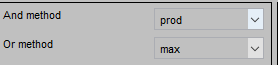
\includegraphics[width=0.7\paperwidth]{sug_params}}
	        	\caption{Выбранные реализации операций.}
	        	\label{sug_params}
	        \end{figure}
	        
			\begin{figure}[h!]
				\center{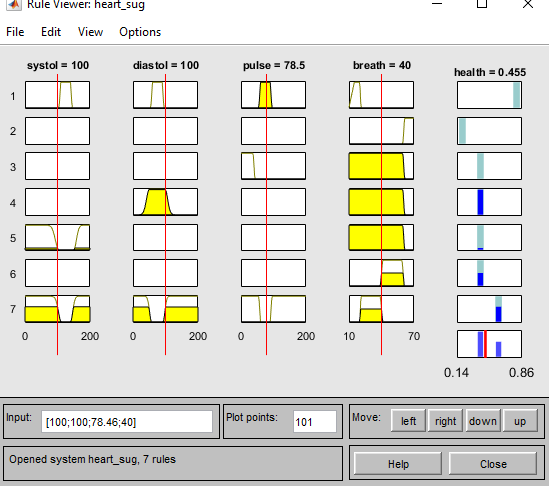
\includegraphics[width=0.6\paperwidth]{sug_wtaver}}
				\caption{Метод взвешенного среднего.}
			\end{figure}
			
			\begin{figure}[h!]
				\center{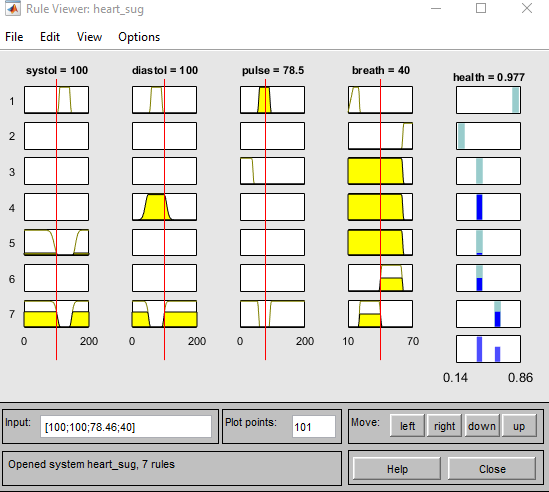
\includegraphics[width=0.6\paperwidth]{sug_wtsum}}
				\caption{Метод взвешенной суммы.}
			\end{figure}
		